%! TEX root = **/010-main.tex
% vim: spell spelllang=en:

\section{Parameter search}%
\label{sec:parameter-search}

A parameter search was performed on the system, to obtain a table that related
the different parameter combinations with the number of limit cycles found.
Given that there where cases where a limit was not detected, the hope was

There where 5 parameters so the search space is quite large even if we only
consider a few possible values. Determining the number of cycles of a system
took~$\approx 1.5$ seconds using a $2048 \times 2048$ grid (depending on the
characteristics of the system).

\subsection{Compactified}

Since there was not enough time to compute a wide search we only applied
variations from the original parameters in \cref{eq:kuznetsov} one at a time.
2500 different values where tried for each parameter (keeping the others as
normal). This gives a total of $2500*5$ different systems to try which at
$1.5$ seconds took around 5 hours and a half. We used tangent compactification
a step size of $1^{-3}$, 20000 steps, tolerance $10^{-6}$ and \emph{Runge Kutta}
of order 3.

\subsection{Not compactified}

We also performed a smaller parameter search without applying compactification
using a window of $x, y \in (-50, 50)$ with the same search configuration.

\pagebreak
\subsection{Results}

\Cref{tab:par} shows the parameter search results for the two searches performed.
Unfortunately non of the searches found 4 or more cycles, which is to be expected since
we only varied one parameter at a time so the system was always quite close to the
original. However it shows that the compactification does obtain more results than
using an arbitrary window.

\begin{table}[H]
    \centering
    \caption{Parameter search results}%
    \label{tab:par}
    \begin{tabular}{ccccc}
        \toprule
        & 2 cycles & 3 cycles & $\geq4$ cycles & Total analyzed\\
        \midrule
        Compactified & 648 & 172 & 0 & 12500 \\
        (-50, 50) & 158 & 119 & 0 & 12500 \\
        \bottomrule
    \end{tabular}
\end{table}

Despite not finding 4 or more limit cycles some of the results where sampled from the
ones obtained to check if indeed they contained the limit cycles specified. In most cases
the number was correct. There were a few exceptions caused by applying the \emph{Kmeans}
on too little points. However these can easily be filtered out by comparing the differences
between the sizes of the cycles found.

\Cref{fig:bounding_c72} shows one of the results that gave limit cycles with
close proportions. This was found in the parameter search using the compactified
plane. In this system all the cycles are closer in size. Note that the changes in the
parameter are minimal.

\begin{figure}[H]
    \centering
    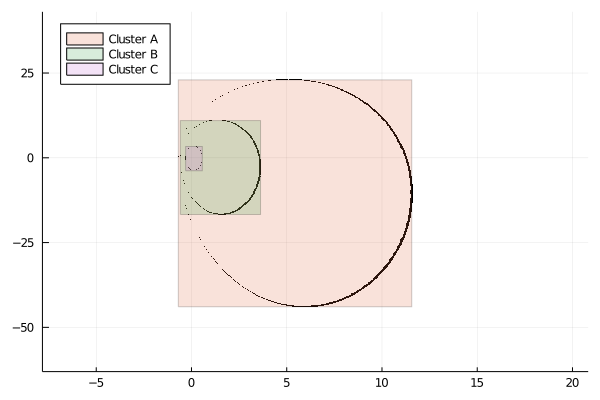
\includegraphics[width=0.8\textwidth]{bounding_c72}
    \caption{Limit cycles found on system from \cref{eq:kuznetsov} \\
        With modified parameter $c=-72.05$
    }%
    \label{fig:bounding_c72}
\end{figure}

In the search all the systems of 3 cycles found where with
very similar values to the ones in \cref{eq:kuznetsov}. The systems with 2 cycles where
much more diverse. In \cref{fig:bounding_left} there is one system in which with
$a=-27.7$ there are 2 limit cycles found, one very small around
the origin is and a much bigger one to the left. This left limit cycle is the
one which with higher parameters of $a$ we cannot detect because it increases
exponentially and the trajectories become unstable. However finding this left cycle
shows that with a capable integrator which can handle stiff trajectories the cycle should
be found in other systems.

\begin{figure}[H]
    \centering
    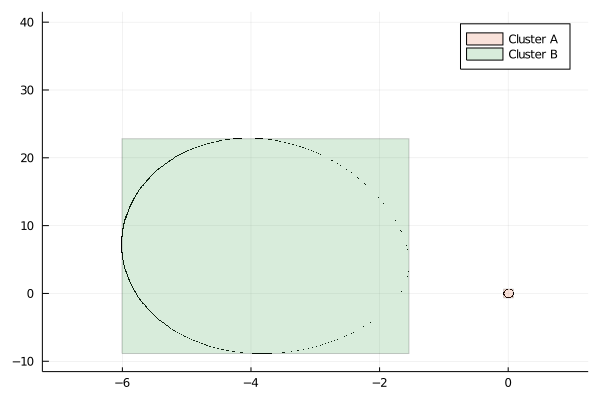
\includegraphics[width=0.8\textwidth]{left_cycle}
    \caption{Limit cycles found on system from \cref{eq:kuznetsov} \\
        With modified parameter $a=-27.7$
    }%
    \label{fig:bounding_left}
\end{figure}
